\section{Complex Numbers}
%
%
%
\label{sec:complessi}

From a geometric perspective, the set $\CC$ of \emph{complex numbers}%
\mymargin{complex numbers}%
\index{numbers!complex}
\index{$\CC$}
can be viewed as a Cartesian representation of the Euclidean plane.
On the plane, we arbitrarily fix a point $0$ (the origin) and arbitrarily fix a
basis $e_1$, $e_2$ of orthonormal vectors.
We identify each point of the plane with the corresponding vectors applied at
$0$. The line generated by the vector $e_1$ is identified with the line $\RR$ of
real numbers, and we set $1=e_1$.
The orthogonal line generated by the vector $e_2$ is called the line of
\emph{imaginary numbers}, and we define $i=e_2$.

A generic point $z$ of the plane $\CC$ can be uniquely expressed in the chosen
basis: $z = x e_1 + y e_2$, or, as we have named $e_1$ and $e_2$:
\[
z = x + i y.
\]
Such $z$ is called a \emph{complex number} with real part $x$ and imaginary part
$y$.
This representation of the complex number $z$ is called the \emph{Cartesian
representation}%
\mymargin{Cartesian representation}%
\index{representation!Cartesian} as it defines the point $z$ of the complex plane through its Cartesian coordinates $x$ and $y$.
Real numbers are \emph{embedded} in the complex numbers, in the sense that if
$x\in \RR$, then $z= x + i\cdot 0 = x$ is also a complex number.
The complex number $i = 0 + i\cdot 1$ is called the \emph{imaginary unit}%
\mymargin{imaginary unit}%
\index{unit!imaginary}
and complex numbers of the form $iy$ are called \emph{imaginary}.
\index{numbers!imaginary}
\index{imaginary}
A complex number $z = x+iy$ is thus a sum of a real number and an imaginary
number. The real number $x$ is called the \emph{real part}
\index{part!real}
of $z$ and is denoted by $x=\Re z$.
\mymargin{$\Re z$}%
\index{$\Re z$}
The real number $y$ is called the \emph{imaginary part}
\index{part!imaginary}
of $z$ and is denoted by $y=\Im z$
\mymargin{$\Im z$}%
\index{$\Im z$}
(note that the imaginary part of a complex number is a real number, not
imaginary). Thus $z= \Re z + i \Im z$.

The set $\CC$, as constructed, is a real vector space of dimension $2$.
We have thus already defined the \emph{addition}%
\mymargin{addition}%
\index{addition}
\index{complex numbers!addition}
between elements of $\CC$ and the multiplication between elements of $\CC$ and
elements of $\RR$.
If $a,b,c,d,t\in \RR$, we have:
\begin{gather*}
 (a+ib) + (c+id) = (a+c) + i (b+d), \\
 t(a+ib) = ta + itb.
\end{gather*}

We wish to extend the \emph{multiplication}%
\mymargin{multiplication}%
\index{multiplication} to all pairs of complex numbers.
\index{complex numbers!multiplication}
By arbitrarily imposing that $i\cdot i = -1$ and that the distributive property
remains valid, we obtain this definition:
\[
   (a+ib) \cdot (c+id) = (ac-bd) + i(ad+bc).
\]

It can be verified that this multiplication extends the previously defined
"scalar" multiplication.
It is also easy to verify that addition and multiplication satisfy the
commutative, associative, and distributive properties, that $0$ is the additive
identity, and that $1$ is the multiplicative identity.
Note that if $z=x+iy$ is non-zero, then
\[
  (x+iy) \cdot \frac{x-iy}{x^2+y^2} = 1.
\]
This means that every $z\neq 0$ has a multiplicative inverse, and thus $\CC$ is
ultimately a field.

Note that no order relation is defined on $\CC$ because it is indeed impossible
to define an order "compatible" with the operations just defined.%
\mynote{%
If $\CC$ were an ordered field, for contradiction, it would have to be that
$z^2\ge 0$ for every $z\in \CC$ (this is true in all ordered fields).
But then $-1 =i^2 \ge 0$, i.e., $1\le 0$, which contradicts the property $0<1$
valid in every ordered field.
} % marginnote

On $\CC$, we define additional operations.
The \emph{conjugate}%
\mymargin{conjugate}%
\index{conjugate}%
\index{complex numbers!conjugation}
of a complex number $z=x+iy$ is the number
$\bar z = x - iy$. Geometrically, the operation of conjugation is a symmetry
with respect to the real line. Real numbers are indeed fixed points of the
conjugation (the conjugate of a real number is the number itself).
It is a simple exercise to verify that conjugation "passes through" addition and
multiplication:
\[
\overline{z+w} = \bar z + \bar w, \qquad
\overline{z\cdot w} = \bar z \cdot \bar w.
\]
Obviously, it holds that $\overline {\bar z} = z$.
It is also useful to observe that:
\begin{equation}\label{eq:re_im}
  \Re z = \frac{z+\bar z}{2}, \qquad
  \Im z = \frac{z-\bar z}{2i}
\end{equation}
and
\[
z \cdot \bar z = (x+iy)(x-iy) = x^2-i^2y^2 = x^2+y^2.
\]

We can then define the
\emph{modulus}%
\mymargin{modulus}%
\index{modulus}%
\index{complex numbers!modulus}
 of a complex number $z=x+iy$
as the real number
\[
\abs{z} = \sqrt{z\cdot\bar z} = \sqrt{x^2+y^2}.
\]
Geometrically, this quantity represents the distance of the point $z$
from the point $0$, and thus the distance between two complex numbers $z$ and
$w$ can be represented by $\abs{z-w}$.

Note that if $z = x \in \RR \subset \CC$, the modulus of $z$ coincides
with the absolute value: $\abs{z} = \sqrt{x^2} = \abs{x}$, and for this
reason, we do not distinguish, in notation, the modulus from the absolute value.
More generally, for every $z\in \CC$, it holds (the verification is immediate):
\[
  \abs{\Re z} \le \abs{z}, \qquad
  \abs{\Im z} \le \abs{z}.
\]

We can now find a useful formula for calculating
the reciprocal of a complex number. Since
$z\cdot \bar z = \abs{z}^2$, we observe that
\[
  \frac{1}{z}
  = \frac{\bar z}{ \bar z \cdot z}
  = \frac{\bar z}{\abs{z}^2}.
\]

\begin{theorem}
The modulus of a complex number satisfies (like the absolute value)
the following properties
\begin{enumerate}
\item $\big\lvert\abs{z}\big\rvert = \abs{z}$,
\item $\abs{-z} = \abs{z}$ = $\abs{\bar z}$,
\item $\abs{z\cdot w} = \abs{z}\cdot\abs{w}$.
\item $\abs{z+w} \le \abs{z}+\abs{w}$ (convexity),
\item $\abs{z-w} \le \abs{z-v} + \abs{v-w}$ (triangle inequality),
\end{enumerate}
\end{theorem}
%
\begin{proof}
The first property is obvious since the absolute value of a non-negative real
number is the number itself.

The second property follows immediately from the definition.

The third property is obtained by observing that 
\[
\abs{z\cdot w}^2 
  = zw \cdot \overline{zw} 
  = z\bar z \cdot w\bar w = \abs{z}^2 \cdot \abs{w}^2 
  = (\abs z \cdot \abs w)^2.
\]
% For the third property, let $z=x+iy$, $w=a+ib$.
% Then:
% \begin{align*}
% \abs{z\cdot w}
% &= \abs{(x+iy)\cdot(a+ib)}
% =\abs{xa - y b+ i(xb + ay)} \\
% &= \sqrt{(xa-yb)^2 + (xb+ay)^2}\\
% &=\sqrt{x^2 a^2 + y^2b^2 - 2xayb + x^2b^2+a^2y^2+2xbay} \\
% &=\sqrt{x^2 a^2 + y^2 b^2 + x^2 b^2 + a^2 y^2}\\
% &=\sqrt{x^2(a^2+b^2) + y^2(a^2+b^2)}\\
% &=\sqrt{(x^2+y^2)(a^2+b^2)}
% =\abs{x+iy} \cdot \abs{a+ib}\\
% &=\abs{z}\cdot\abs{w}.
% \end{align*}

For the fourth inequality, observe that
\[
  \abs{z+w}^2 = (z+w)\cdot(\bar z + \bar w)
  = \abs{z}^2 + \abs{w}^2 + z\cdot \bar w + \bar z \cdot w
\]
and since
\[
  z\cdot \bar w + \bar z \cdot w
  = z \cdot \bar w + \overline{z \cdot \bar w}
  = 2 \Re(z\bar w)
  \le 2 \abs {z\bar w}
  = 2 \abs{z}\cdot\abs{\bar w}
  = 2 \abs{z}\cdot\abs{w}
\]
we obtain
\[
 \abs{z+w}^2 \le \abs{z}^2+\abs{w}^2 + 2 \abs{z}\cdot\abs{w}
 =\enclose{\abs z + \abs w}^2
\]
which is equivalent to the convexity inequality.

The triangle inequality is equivalent to convexity, indeed
\[
  \abs{z-w} = \abs{(z-v) + (v-w)}
  \le \abs{z-v} + \abs{v-w}.
\]
\end{proof}

\begin{figure}
  \begin{center}
    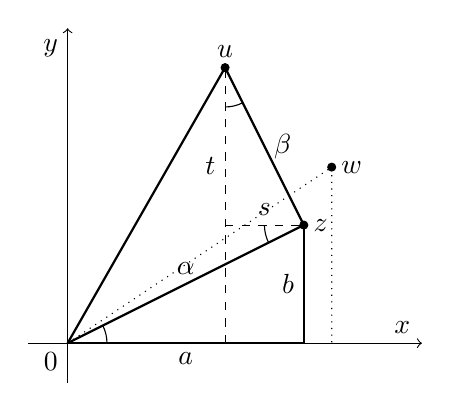
\begin{tikzpicture}[x=0.5cm,y=0.5cm]
    	\draw[->] (-1,0) -- (9,0);
      \draw[->] (0,-1) -- (0,8);
      %
      \draw[dotted] (0,0) -- ({sqrt(45)},{sqrt(20)}) -- ({sqrt(45)},0);
      \draw[fill] ({sqrt(45)},{sqrt(20)}) node[right] {$w$} circle [radius=0.1];
      %
      \draw[thick] (0,0) -- (6,0);
      \draw[thick] (0,0) -- (6,3);
      \draw[thick] (0,0) -- (4,7);
      \draw[thick] (6,0) -- (6,3);
      \draw[thick] (6,3) -- (4,7);
      %
      \draw[dashed] (4,0) -- (4,7);
      \draw[dashed] (4,3) -- (6,3);
      %
      \draw (1,0) arc (0:{atan(1/2)}:1);
      \draw (6,3)+(-1,0) arc (180:{180+atan(1/2)}:1);
      \draw (4,7)+(0,-1) arc (-90:{-90+atan(1/2)}:1);
      %
      \draw[fill] (6,3) node[right] {$z$} circle [radius=0.1];
      \draw[fill] (4,7) node[above] {$u$} circle [radius=0.1];
      %
      \node[below] at (3,0) {$a$};
      \node[left] at (6,1.5) {$b$};
      \node[above] at (3,1.5) {$\alpha$};
      \node[right] at (5,5) {$\beta$};
      \node[above] at (5,3) {$s$};
      \node[left] at (4,4.5) {$t$};
      \node[above] at (8.5,0) {$x$};
      \node[left] at (0,7.5) {$y$};
      \node[below left] at (0,0) {$0$};
    \end{tikzpicture}
  \end{center}
  \caption{Consider the complex numbers $z=a+ib$ and $w=\alpha+i\beta$
  and suppose that $\alpha^2 = a^2+b^2$.
  Consider the point $u$ obtained by rotating the point $w$ by the angle
  determined by the point $z$. Then $u=a-s + i(b+t)$ where $s$ and $t$
  are the legs of the right triangle with hypotenuse $\beta$.
  Thanks to the properties of similar triangles, we have
  $\frac{s}{\beta} = \frac{b}{\alpha}$ and $\frac{t}{\beta} = \frac{a}{\alpha}$
  from which we obtain $u = a-\frac{b\beta}{\alpha}+i(b+\frac{a\beta}{\alpha})$
  or $\alpha u = (a\alpha - b \beta) + i (b\alpha + a \beta) = z\cdot w$.
  This means that the complex number $z\cdot w$ lies on the ray
  that determines an angle which is the sum of the angles determined
  by the complex numbers $z$ and $w$.
  }
  \label{fig:prodotto_complesso}
\end{figure}

We can now provide a geometric interpretation of the product $z\cdot w$
between two complex numbers. First, we know that $\abs{z\cdot w} = \abs{z} \cdot
\abs{w}$, and thus the point on the plane representing the product $z\cdot w$ is
at a distance from the origin equal to the product of the distances of the
points $z$ and $w$. Moreover, the angle determined by $z\cdot w$ with respect to
the positive $x$-axis is equal to the sum of the angles determined by the points
$z$ and $w$, as shown in Figure~\ref{fig:prodotto_complesso}.

The plane of complex numbers can also be extended by adding a point at
\emph{infinity}%
\mymargin{infinity}%
\index{infinity}.
Unlike the real numbers, where there was an order that was useful to preserve,
in the case of complex numbers, it is more common to use a single point at
infinity denoted by \emph{$\infty$}%
\mymargin{$\infty$}%
\index{$\infty$}.
We define the set of extended complex numbers $\bar \CC$ as
\[
\bar \CC = \CC \cup \ENCLOSE{\infty}.
\]
We define
\begin{align*}
  z + \infty &= \infty \qquad \forall z \in \CC\\
  z - \infty &= \infty \qquad \forall z \in \CC\\
   z\cdot \infty &= \infty \qquad \forall z \in \bar\CC\setminus\ENCLOSE{0} \\
   z / \infty &= 0 \qquad \forall z \in \CC \\
   z / 0 &= \infty \qquad \forall z \in \bar \CC \setminus\ENCLOSE{0}\\
   \bar \infty &= \infty \\
   \abs{\infty} &= +\infty \in \bar \RR.
\end{align*}
Note that we have defined division by zero for complex numbers
(and thus also real numbers) different from zero. The result is $\infty$,
confirming that division by zero is not a valid operation if we want a finite
result.
A quantity $z\in \bar \CC$ will be said to be \emph{finite} if $z\in \CC$.

\begin{example}
  The function $f\colon \bar \CC \to \bar \CC$ 
  defined by 
  \[
  f(z) = \frac{1}{z}
  \]
  is a bijective function from $\bar \CC$ to itself.
  From a geometric perspective, the conjugate of this function,
  namely the function $z\mapsto \frac 1 {\bar z}$, 
  is the circular inversion with respect to the unit circle of $\CC$:
  points on the unit circle are left fixed,
  points inside are mapped outside while remaining on the 
  same ray emanating from the origin and inverting their modulus.
  The points $0$ and $\infty$ are exchanged.
\end{example}

%% % ancora non abbiamo definito il concetto di funzione continua
%% Per le funzioni di variabile complessa e/o a valori complessi 
%% si applica la stessa definizione~\ref{def:continua} di continuità 
%% che abbiamo dato per le funzioni reali utilizzando il modulo 
%% complesso al posto del valore assoluto.
%% \index{continuità!campo complesso}%
%% \index{funzione!continua!complessa}%

\begin{exercise}
  \label{ex:radice_uno}
Solve, in the complex field, the equation 
\[
  z^2=1.
\]
\end{exercise}
\begin{proof}[Solution.]
Let $z=x+iy$ with $x,y\in \RR$, we obtain 
$x^2-y^2 + 2 i xy = 1$, from which, equating the real part 
and the imaginary part, we obtain $x^2-y^2=1$, $xy=0$.
It cannot be $x=0$, otherwise we would have $y^2=-1$
which has no solution $y\in \RR$.
Thus it must be $y=0$, from which we obtain $x^2=1$ and hence $x=\pm 1$.

Thus the equation has two solutions: $z=1$ and $z=-1$.
\end{proof}
\begin{exercise}
  \label{ex:radice_quarta_uno}
Solve, in the complex field, the equation
\[
  z^4 = 1.
\]
\end{exercise}
\begin{proof}[Solution.]
Let $w=z^2$, the equation becomes $w^2=1$.
From the previous exercise, we know that it must be 
$w=\pm 1$.
If $w=1$, we have, in turn, $z^2=1$ and thus $z=\pm 1$, as above.
If instead $w=-1$, we have $z^2=-1$, that is, 
multiplying both sides by $i^2=-1$,
$(iz)^2=1$, from which $iz=\pm 1$, or $z=\pm i$.

We thus have four solutions: $z=1,i,-1,-i$.
\end{proof}

\begin{exercise}[square root]
  \label{ex:radice_complessa}
Given $c\in \ZZ$, the equation
\[
z^2 = c
\]
has two solutions $z_1,z_2\in \CC$ with $z_2=-z_1$ if $c\neq 0$ 
and has a single solution $z=0$ if $c=0$.
\end{exercise}
\begin{proof}[Solution.]
If $z^2=c$, taking the modulus of both sides, we obtain 
$\abs{z}^2=\abs{c}$, from which $\abs{z}=\sqrt{\abs c}$.
Thus if $c=0$, it must be $\abs{z}=0$, leading to the unique
solution $z=0$.

If $c\neq 0$, we can set $z=x+iy$ and $c=a+ib$
with $x,y,a,b\in \RR$.
If $z^2=c$, we will have $\abs{z}=\sqrt{\abs c}$
and $(x+iy)^2 = x^2 - y^2 + 2ixy = a + ib$. 
Thus $a=x^2-y^2 = 2x^2 - \abs{z}^2 = 2x^2- \abs{c}$ 
and similarly $a = \abs{c}-2y^2$, from which 
\[
  x = \pm \sqrt{\frac{\abs{c}+a}2}, \qquad
  y = \pm \sqrt{\frac{\abs{c}-a}2}.
\]
Note that $\abs{a}\le \abs{c}$, so the arguments of the 
square roots are real non-negative.
The two signs $\pm$ cannot be chosen arbitrarily, 
the condition $b=2xy$ imposes a relation between the two signs
(concordant if $b>0$, discordant if $b<0$, if $b=0$, we have $y=0$ 
and only the sign of $x$ remains).

Since $x$ and $y$ cannot both be zero, we always have
two opposite solutions.
\end{proof}

\begin{exercise}[bisection]
\label{ex:bisezione}
Verify that if $\abs{z}=1$, then
\[
  \enclose{\frac{z+1}{\abs{z+1}}}^2 = z. 
\]
\end{exercise}
\begin{proof}[Solution.]
Recalling that $z \bar z = \abs{z}^2 = 1$ 
and thus $\frac 1 z = \bar z$, we obtain
\[
  \enclose{\frac{z+1}{\abs{z+1}}}^2
  = \frac{z^2+2z+1}{(z+1)(\bar z+1)}
  = z\cdot \frac{z + 2 + \bar z} {z\bar z + z + \bar z + 1}
  =z.
\]
\end{proof}

\begin{exercise}[vertices of an equilateral triangle]
Solve the equation 
\[ 
 z^3 - 1 = 0
\]
in the complex field.
\end{exercise}
%
\begin{proof}[Solution.]
Recall the notable product:
\[
  z^3 - 1 = (z-1)(z^2+z+1).
\]
Thus $z=1$ is a solution, and the other solutions must solve 
the equation $z^2+z+1=0$. 
Certainly, $z=0$ is not a solution, and thus we can divide by $z$ 
and obtain:
\[
  z + 1 + \frac 1 z = 0.
\]
Now observe that if $z$ is a solution, we have $1=z^3$
and thus: $1 = \abs{z^3}= \abs{z}^3$, from which $\abs z = 1$.
But then $z\cdot \bar z = \abs{z}^2 = 1$, i.e., $\frac 1 z = \bar z$.
Thus we have 
\[
    z + 1 + \bar z = 0.
\]
But if $z=x+iy$ with $x,y\in \RR$, then $z+\bar z = 2x$
and thus 
\[
    2x + 1 = 0 
\]
from which $x=-\frac 1 2$. Moreover, since $x^2+y^2=\abs{z}^2=1$, we obtain
$y^2 = 1-x^2 = \frac 3 4$, from which $y=\pm \frac{\sqrt 3}{2}$.

The given equation thus has $3$ solutions:
\[
z_0 = 1, \qquad 
z_{1,2} = -\frac 1 2 \pm i \frac{\sqrt 3} 2.
\]

These three points, when plotted on the Gaussian plane, are 
at the vertices of an equilateral triangle inscribed in the unit circle.
Indeed, the geometric interpretation of the product of complex numbers tells us 
that the point $z_1$ determines on the Gaussian plane an angle equal 
to one-third of a full circle. Moreover, we have $z_2 = z_1^2$, and thus 
$z_2$ corresponds to $\frac 2 3$ of a full circle, and $z_0=z_1^3 = 1$
represents
the full circle (or the null angle).
\end{proof}

\begin{exercise}[regular pentagon]
Determine the maximum distance between two solutions 
of the equation $z^5=1$. 
\end{exercise}

%%%%%%%%%%%%%%%%%%%%%%%%%%%%%%%%%%%%%%%%%%
%%%%%%%%%%%%%%%%%%%%%%%%%%%%%%%%%%%%%%%%%%
%%%%%%%%%%%%%%%%%%%%%%%%%%%%%%%%%%%%%%%%%%